% ============================================================================
% ATIVIDADE 8
%
% Este capitulo utiliza TikZ nos diagramas.
% Caso ainda nao esteja no preambulo do relatorio, adicionar:
%
% \usepackage{tikz}
%
% O codigo-fonte e carregado por \lstinputlisting e pressupoe que o estilo
% "codigoC" ja esteja definido no preambulo geral do relatorio.
% ============================================================================

\chapter{Atividade 8 -- Paralelismo de tarefas, paralelismo de dados e regiões paralelas aninhadas}

\label{chap:atvd08}

% ============================================================================
\section{Enunciado da tarefa}
\label{sec:atvd08-enunciado}
% ============================================================================

\begin{quote}
Implemente um código em OpenMP que realize as seguintes tarefas:

\begin{enumerate}
    \item inicialize um vetor que representa uma função qualquer, gerando os
    valores necessários para o seu processamento;
    \item calcule a integral desse vetor utilizando o método do trapézio;
    \item calcule o vetor que representa a derivada do vetor utilizando o
    método de diferenças finitas.
\end{enumerate}

As tarefas que não possuem dependência entre si devem ser executadas em
paralelo utilizando a diretiva \texttt{sections}. Cada tarefa deve utilizar
pelo menos duas threads para realizar seu processamento. Após a conclusão de
cada tarefa, o resultado correspondente deve ser impresso por apenas uma
thread.

Ao final, devem ser discutidas as funcionalidades do OpenMP utilizadas na
implementação, considerando:

\begin{itemize}
    \item como foi explorado o paralelismo de tarefas;
    \item como foi explorado o paralelismo de dados, distribuindo o
    processamento entre múltiplas threads;
    \item quais recursos do OpenMP foram utilizados para permitir o
    aninhamento de regiões paralelas;
    \item quais diretivas ou mecanismos foram utilizados para garantir que
    determinadas operações, como a impressão dos resultados, fossem
    executadas por apenas uma thread;
    \item quais mecanismos de sincronização estão presentes no código e qual
    é a função de cada um.
\end{itemize}
\end{quote}


% ============================================================================
\section{Objetivos e requisitos}
\label{sec:atvd08-objetivos}
% ============================================================================

A atividade tem como objetivo principal integrar, em uma única implementação,
dois níveis distintos de paralelismo em OpenMP. No nível externo, operações
independentes devem ser tratadas como tarefas distintas e executadas
concorrentemente. No nível interno, o processamento de cada tarefa deve ser
distribuído entre múltiplas threads.

A solução desenvolvida foi orientada pelos seguintes requisitos:

\begin{itemize}
    \item representar numericamente uma função por meio de um vetor;
    \item realizar a inicialização desse vetor utilizando duas threads;
    \item calcular uma aproximação numérica da integral pelo método composto
    dos trapézios;
    \item calcular uma aproximação da derivada por diferenças finitas;
    \item executar integral e derivada como tarefas independentes utilizando
    \texttt{sections};
    \item empregar pelo menos duas threads no processamento interno de cada
    tarefa;
    \item habilitar explicitamente o paralelismo aninhado;
    \item utilizar um mecanismo seguro para a acumulação da integral;
    \item garantir que a apresentação final dos resultados seja realizada
    por apenas uma thread;
    \item validar numericamente os resultados por comparação com soluções
    analíticas conhecidas;
    \item tornar visíveis, no terminal, tanto as threads externas responsáveis
    pelas \texttt{sections} quanto as equipes internas utilizadas por cada
    tarefa.
\end{itemize}

A atividade não foi tratada como um estudo de desempenho. Não foram definidos
speedup, eficiência, escalabilidade ou comparação temporal entre versões
sequenciais e paralelas. O foco foi a demonstração funcional das construções
de OpenMP solicitadas no enunciado.


% ============================================================================
\section{Fundamentação conceitual}
\label{sec:atvd08-fundamentacao}
% ============================================================================

\subsection{Particionamento de tarefas e de dados}

A paralelização de um problema pode ocorrer em níveis diferentes. No
\textit{paralelismo de tarefas}, operações funcionalmente distintas e sem
dependências entre si são executadas simultaneamente. No \textit{paralelismo
de dados}, uma mesma operação é aplicada simultaneamente a diferentes
partições de um conjunto de dados.

Nesta atividade, os dois modelos aparecem em conjunto. Uma vez concluída a
inicialização do vetor, o cálculo da integral não depende do resultado da
derivada, e o cálculo da derivada não depende do resultado da integral.
Portanto, essas duas operações constituem tarefas independentes.

Pode-se representar essa dependência por

\[
\text{Inicialização}
\longrightarrow
\begin{cases}
    \text{Integral},\\
    \text{Derivada}.
\end{cases}
\]

A inicialização precisa necessariamente ocorrer primeiro, pois ambas as
tarefas subsequentes utilizam os valores armazenados no vetor da função.

No interior de cada tarefa, entretanto, existem muitas operações independentes
sobre diferentes elementos do vetor. Essas operações podem ser distribuídas
entre múltiplas threads, caracterizando paralelismo de dados.


\subsection{Representação discreta da função}

Foi escolhida a função

\[
f(x)=x^2
\]

no intervalo

\[
[a,b]=[0,10].
\]

O domínio foi discretizado em

\[
N=100000
\]

pontos igualmente espaçados.

O espaçamento é dado por

\[
h=\frac{b-a}{N-1},
\]

de modo que

\[
h=\frac{10}{99999}
\approx
0{,}00010000100001.
\]

Para cada posição $i$ do vetor,

\[
x_i=a+ih
\]

e

\[
y_i=f(x_i)=x_i^2.
\]

A escolha de $f(x)=x^2$ foi deliberadamente simples, pois permite validar tanto
a integral quanto a derivada contra expressões analíticas conhecidas, sem
introduzir complexidade matemática desnecessária ao objetivo principal da
atividade.


\subsection{Método composto dos trapézios}

Para uma função discretizada em pontos igualmente espaçados, o método
composto dos trapézios fornece

\[
I_T
=
h
\left[
\frac{y_0}{2}
+
\sum_{i=1}^{N-2} y_i
+
\frac{y_{N-1}}{2}
\right].
\]

O termo

\[
\sum_{i=1}^{N-2}y_i
\]

pode ser particionado entre diferentes threads. Entretanto, como todas as
threads contribuem para o mesmo acumulador lógico, uma atualização direta de
uma variável compartilhada produziria uma condição de corrida.

A construção de redução do OpenMP resolve esse problema criando acumuladores
privados e combinando-os ao final da região de trabalho. Por isso, foi
utilizada a cláusula

\begin{center}
\texttt{reduction(+:sum)}.
\end{center}

Para a função adotada, a solução analítica é

\[
I
=
\int_0^{10}x^2\,dx
=
\left[\frac{x^3}{3}\right]_0^{10}
=
\frac{1000}{3},
\]

portanto

\[
I
\approx
333{,}333333333333.
\]


\subsection{Derivação por diferenças finitas}

Para os pontos internos do domínio foi utilizada a diferença central

\[
f'(x_i)
\approx
\frac{y_{i+1}-y_{i-1}}{2h},
\qquad
1\leq i\leq N-2.
\]

Como esse esquema necessita de elementos dos dois lados do ponto avaliado,
ele não pode ser aplicado diretamente às extremidades.

No primeiro ponto foi utilizada a diferença progressiva

\[
f'(x_0)
\approx
\frac{y_1-y_0}{h},
\]

enquanto no último ponto foi utilizada a diferença regressiva

\[
f'(x_{N-1})
\approx
\frac{y_{N-1}-y_{N-2}}{h}.
\]

Para

\[
f(x)=x^2,
\]

a derivada analítica é

\[
f'(x)=2x.
\]

Além de facilitar a validação, a função quadrática possui uma característica
útil: no interior do domínio, a diferença central recupera exatamente $2x$
em aritmética exata, pois

\[
\frac{(x+h)^2-(x-h)^2}{2h}
=
\frac{4xh}{2h}
=
2x.
\]


\subsection{Diretiva \texttt{sections}}

A construção \texttt{sections} é apropriada quando diferentes blocos de
código podem executar independentemente. Cada bloco delimitado por
\texttt{section} é atribuído a uma thread da equipe externa.

Nesta atividade foram definidas duas seções:

\[
\texttt{section}_1
\longrightarrow
\text{integral}
\]

e

\[
\texttt{section}_2
\longrightarrow
\text{derivada}.
\]

Não foi estabelecida uma associação fixa entre uma determinada thread e uma
determinada seção. Essa decisão é deixada ao runtime do OpenMP.


\subsection{Paralelismo aninhado}

Uma \texttt{section} é executada por uma única thread da região que contém a
construção \texttt{sections}. Entretanto, o enunciado exige que cada tarefa
utilize pelo menos duas threads em seu processamento.

Por esse motivo, cada \texttt{section} cria uma nova região paralela interna.
A estrutura lógica passa a ser

\[
\text{região paralela externa}
\rightarrow
\texttt{sections}
\rightarrow
\text{região paralela interna}.
\]

Consequentemente, são explorados dois níveis distintos:

\[
\boxed{\text{nível externo: paralelismo de tarefas}}
\]

e

\[
\boxed{\text{nível interno: paralelismo de dados}}.
\]

O código habilita explicitamente o paralelismo aninhado por meio de

\begin{center}
\texttt{omp\_set\_nested(1)}.
\end{center}

Também é utilizado

\begin{center}
\texttt{omp\_set\_dynamic(0)},
\end{center}

evitando que o runtime reduza dinamicamente o número de threads solicitado
durante esta demonstração.


\subsection{Sincronização}

Não foi necessário inserir uma diretiva \texttt{barrier} explícita. A
sincronização da solução é obtida principalmente por pontos de sincronização
implícitos das construções OpenMP utilizadas.

Ao final da região paralela responsável pela inicialização, todas as threads
foram concluídas antes que o programa avance para as tarefas que consomem o
vetor.

No interior das tarefas, o término das regiões paralelas internas garante que
o processamento distribuído tenha sido concluído antes da continuação da
thread que criou aquela região.

A construção \texttt{sections}, sem a cláusula \texttt{nowait}, possui uma
barreira implícita ao final. Assim, quando a execução alcança a etapa de
impressão, tanto a integral quanto a derivada já foram finalizadas.

Finalmente, a diretiva \texttt{single} garante que apenas uma thread da equipe
externa execute o bloco responsável pela apresentação consolidada dos
resultados.


\subsection{\texttt{single}, \texttt{master} e a escolha adotada}

A diretiva \texttt{single} permite que uma única thread qualquer da equipe
execute determinado bloco. Já a construção \texttt{master} restringe a
execução especificamente à thread mestre.

Como o requisito da atividade exige apenas que a impressão seja feita por uma
única thread, e não necessariamente pela thread de identificador zero, foi
adotado \texttt{single}.

Além disso, essa decisão evita impor uma associação artificial entre
``impressão'' e ``thread 0'', preservando a semântica de que qualquer thread
da equipe pode assumir a responsabilidade pela operação serial.


% ============================================================================
\section{Interpretação didática da tarefa}
\label{sec:atvd08-interpretacao}
% ============================================================================

A atividade não consiste apenas em calcular uma integral e uma derivada
numericamente. Esses cálculos funcionam como um problema simples sobre o qual
podem ser demonstrados diferentes mecanismos de paralelização.

A inicialização mostra uma decomposição de dados elementar: diferentes
threads escrevem em índices distintos do mesmo vetor.

Em seguida, integral e derivada representam duas funções computacionais
diferentes que podem ser executadas simultaneamente. Essa etapa demonstra
paralelismo de tarefas.

Cada uma dessas tarefas contém, por sua vez, quantidade suficiente de trabalho
independente para ser novamente paralelizada. A integral distribui os termos
do somatório entre as threads internas, enquanto a derivada distribui os
índices do vetor de saída.

Assim, a atividade constrói a seguinte hierarquia conceitual:

\[
\boxed{
\text{paralelismo de tarefas}
+
\text{paralelismo de dados}
+
\text{paralelismo aninhado}
}.
\]

A impressão dos identificadores das equipes no terminal foi incluída para
tornar essa hierarquia diretamente observável durante a execução, sem
transformar a saída em um log de todas as iterações.


% ============================================================================
\section{Modelagem da solução}
\label{sec:atvd08-modelagem}
% ============================================================================

\subsection{Estrutura geral}

Foram utilizados dois vetores de valores do tipo \texttt{double}:

\[
y[N]
\]

para armazenar a função discretizada, e

\[
dy[N]
\]

para armazenar a derivada numérica.

A configuração consolidada foi:

\begin{table}[htbp]
    \centering
    \caption{Configuração adotada na Atividade 8.}
    \label{tab:atvd08-configuracao}
    \begin{tabular}{|p{0.42\textwidth}|p{0.42\textwidth}|}
        \hline
        \textbf{Parâmetro} & \textbf{Configuração} \\
        \hline
        Função & $f(x)=x^2$ \\
        \hline
        Intervalo & $[0,10]$ \\
        \hline
        Número de pontos & $100000$ \\
        \hline
        Tipo numérico & \texttt{double} \\
        \hline
        Threads na inicialização & 2 \\
        \hline
        Threads na região de \texttt{sections} & 2 \\
        \hline
        Threads internas por tarefa & 2 \\
        \hline
        Integral & método composto dos trapézios \\
        \hline
        Derivada interna & diferença central \\
        \hline
        Bordas da derivada & diferenças progressiva e regressiva \\
        \hline
        Acumulação da integral & \texttt{reduction} \\
        \hline
        Impressão consolidada & \texttt{single} \\
        \hline
        Paralelismo aninhado & habilitado \\
        \hline
        Medição de tempo & não realizada \\
        \hline
    \end{tabular}
\end{table}


\subsection{Dependências}

A dependência principal da aplicação é

\[
\text{inicialização do vetor}
\rightarrow
\{\text{integral},\text{derivada}\}.
\]

Integral e derivada podem começar somente depois que todos os elementos de
$y$ estiverem disponíveis.

Após essa condição ser satisfeita,

\[
\text{integral}
\perp
\text{derivada},
\]

isto é, não existe dependência de dados entre as duas operações.

Elas podem, portanto, ser processadas simultaneamente.


\subsection{Principais funções e componentes}

A implementação foi organizada em funções pequenas, cada uma responsável por
uma etapa bem definida.

\begin{description}

    \item[\texttt{initialize\_vector}]
    Inicializa o vetor $y$ em uma região paralela com duas threads. Cada
    iteração calcula $x_i$ e armazena $x_i^2$.

    \item[\texttt{compute\_integral}]
    Executa o somatório interno do método dos trapézios em uma região
    paralela aninhada. A soma é combinada por meio de
    \texttt{reduction(+:sum)}.

    \item[\texttt{compute\_derivative}]
    Calcula os pontos internos da derivada utilizando um laço paralelo e
    diferença central. As duas extremidades são calculadas separadamente por
    diferenças unilaterais.

    \item[\texttt{print\_seen\_threads}]
    Apresenta os identificadores das threads que participaram de determinada
    equipe.

    \item[\texttt{print\_derivative\_samples}]
    Exibe cinco posições representativas da derivada em vez de imprimir os
    $100000$ elementos do vetor.

    \item[\texttt{main}]
    Configura o problema, aloca os vetores, habilita o paralelismo aninhado,
    inicia as etapas de processamento e realiza a apresentação consolidada dos
    resultados.

\end{description}

As estruturas \texttt{InitInfo} e \texttt{TaskInfo} foram empregadas apenas
para registrar informações necessárias à demonstração didática das equipes de
threads no terminal.


% ============================================================================
\section{Decisões de projeto e trade-offs}
\label{sec:atvd08-decisoes}
% ============================================================================

As principais decisões adotadas são resumidas na
Tabela~\ref{tab:atvd08-decisoes}.

\begin{table}[htbp]
    \centering
    \small
    \caption{Principais decisões de projeto da Atividade 8.}
    \label{tab:atvd08-decisoes}
    \begin{tabular}{
        |p{0.19\textwidth}
        |p{0.22\textwidth}
        |p{0.43\textwidth}|}
        \hline
        \textbf{Aspecto} &
        \textbf{Escolha} &
        \textbf{Justificativa e trade-off} \\
        \hline

        Função &
        $f(x)=x^2$ &
        Permite validação analítica direta da integral e da derivada. A
        simplicidade matemática favorece o foco em OpenMP, embora não
        represente um problema numérico complexo. \\
        \hline

        Número de pontos &
        $N=100000$ &
        Fornece quantidade suficiente de iterações para demonstrar a divisão
        dos dados, mantendo baixo custo de memória. \\
        \hline

        Tipo &
        \texttt{double} &
        Adequado ao cálculo numérico da integral e da derivada e mais preciso
        que \texttt{float}, ao custo de maior uso de memória por elemento. \\
        \hline

        Tarefas &
        duas \texttt{sections} &
        Reflete diretamente a independência entre integral e derivada. O
        número de tarefas é fixo no código, característica inerente ao uso
        de \texttt{sections}. \\
        \hline

        Paralelismo interno &
        duas threads por tarefa &
        Satisfaz explicitamente o requisito do enunciado e mantém simples a
        visualização do paralelismo aninhado. \\
        \hline

        Integral &
        \texttt{reduction} &
        Evita condição de corrida sem serializar cada atualização por
        \texttt{critical} ou \texttt{atomic}. \\
        \hline

        Derivada &
        escrita por índice &
        Cada iteração escreve em uma posição distinta de \texttt{dy}, não
        sendo necessário mecanismo de exclusão mútua. \\
        \hline

        Impressão &
        \texttt{single} &
        Atende ao requisito de uma única thread sem exigir especificamente a
        thread mestre. \\
        \hline

        \texttt{nowait} &
        não utilizado &
        A barreira ao final de \texttt{sections} é útil porque a impressão
        consolidada deve ocorrer somente depois das duas tarefas. \\
        \hline

        Identificação das threads &
        exibida de forma resumida &
        Torna observável a estrutura paralela sem imprimir mensagens por
        iteração, o que poluiria o terminal e introduziria E/S excessiva. \\
        \hline

        Temporização &
        não utilizada &
        O enunciado não solicita benchmark. Evita interpretar uma única
        configuração como estudo de desempenho. \\
        \hline

    \end{tabular}
\end{table}

A opção por \texttt{reduction}, em particular, elimina a necessidade de uma
região crítica para cada termo da soma. Uma implementação baseada em
\texttt{critical} preservaria a correção, mas introduziria serialização
desnecessária justamente na operação que deveria explorar paralelismo.

Da mesma forma, não foi utilizado \texttt{atomic} no vetor de derivadas,
porque as threads escrevem em posições distintas. Adicionar sincronização
nesse caso não aumentaria a correção e apenas acrescentaria sobrecarga.


% ============================================================================
\section{Representação estrutural da implementação}
\label{sec:atvd08-estrutura}
% ============================================================================

A Figura~\ref{fig:atvd08-estrutura} representa os principais componentes da
implementação.

\begin{figure}[htbp]
    \centering

    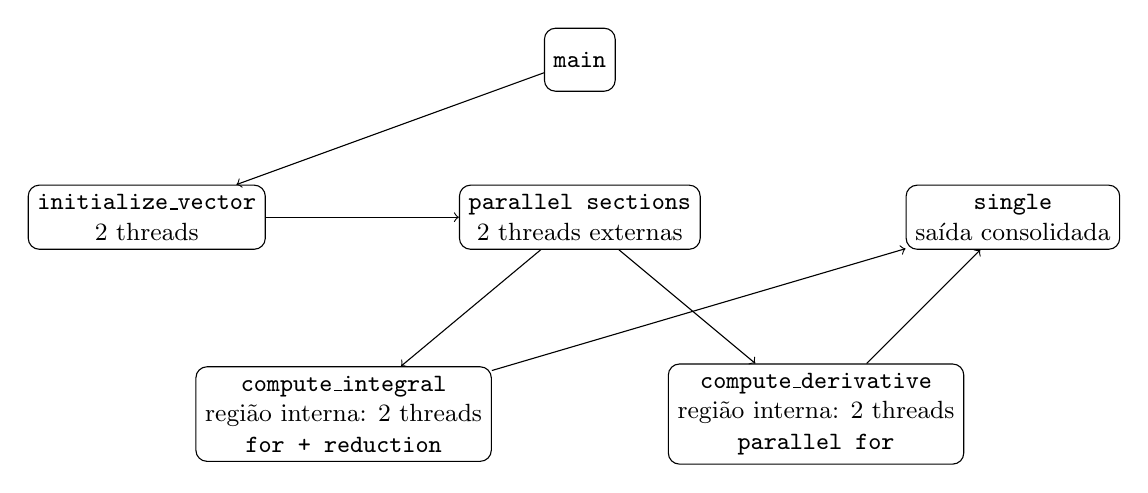
\begin{tikzpicture}[
        every node/.style={
            draw,
            rounded corners,
            align=center,
            minimum height=0.8cm,
            font=\small
        }
    ]

        \node (main) at (0,0)
        {\texttt{main}};

        \node (init) at (-5.5,-2)
        {\texttt{initialize\_vector}\\
         2 threads};

        \node (sections) at (0,-2)
        {\texttt{parallel sections}\\
         2 threads externas};

        \node (output) at (5.5,-2)
        {\texttt{single}\\
         saída consolidada};

        \node (integral) at (-3,-4.5)
        {\texttt{compute\_integral}\\
         região interna: 2 threads\\
         \texttt{for + reduction}};

        \node (derivative) at (3,-4.5)
        {\texttt{compute\_derivative}\\
         região interna: 2 threads\\
         \texttt{parallel for}};

        \draw[->] (main) -- (init);
        \draw[->] (init) -- (sections);
        \draw[->] (sections) -- (integral);
        \draw[->] (sections) -- (derivative);
        \draw[->] (integral) -- (output);
        \draw[->] (derivative) -- (output);

    \end{tikzpicture}

    \caption{Representação estrutural da implementação da Atividade 8.}
    \label{fig:atvd08-estrutura}
\end{figure}

A estrutura evidencia que \texttt{sections} constitui o nível de
paralelismo de tarefas, enquanto as regiões criadas em
\texttt{compute\_integral} e \texttt{compute\_derivative} constituem o nível
interno de paralelismo de dados.


% ============================================================================
\section{Fluxo de execução}
\label{sec:atvd08-fluxo}
% ============================================================================

O fluxo comportamental da aplicação é mostrado na
Figura~\ref{fig:atvd08-fluxo}.

\begin{figure}[htbp]
    \centering

    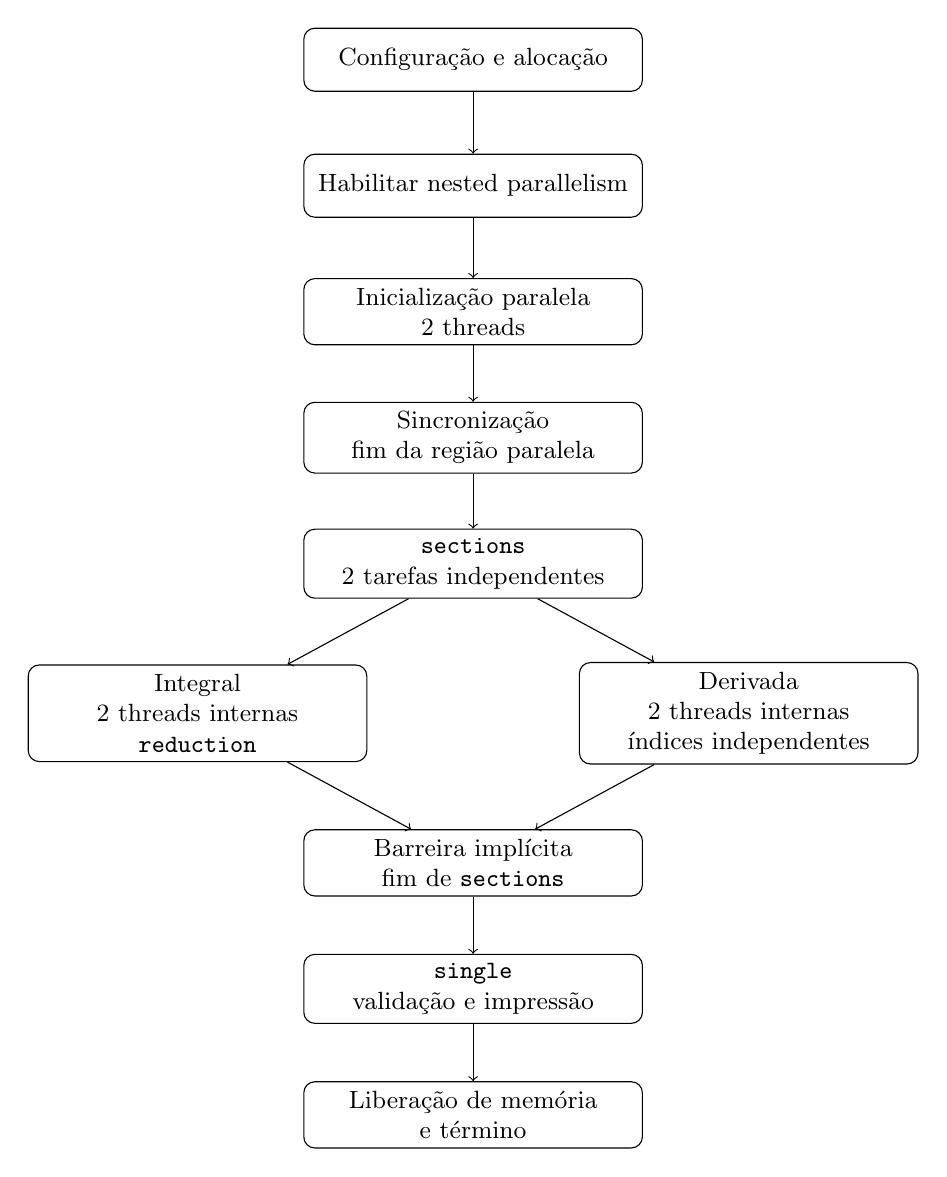
\begin{tikzpicture}[
        every node/.style={
            draw,
            rounded corners,
            align=center,
            minimum height=0.8cm,
            minimum width=4.3cm,
            font=\small
        }
    ]

        \node (start) at (0,0)
        {Configuração e alocação};

        \node (nested) at (0,-1.6)
        {Habilitar nested parallelism};

        \node (init) at (0,-3.2)
        {Inicialização paralela\\2 threads};

        \node (sync1) at (0,-4.8)
        {Sincronização\\fim da região paralela};

        \node (sections) at (0,-6.4)
        {\texttt{sections}\\2 tarefas independentes};

        \node (integral) at (-3.5,-8.3)
        {Integral\\2 threads internas\\\texttt{reduction}};

        \node (derivative) at (3.5,-8.3)
        {Derivada\\2 threads internas\\índices independentes};

        \node (sync2) at (0,-10.2)
        {Barreira implícita\\fim de \texttt{sections}};

        \node (single) at (0,-11.8)
        {\texttt{single}\\validação e impressão};

        \node (end) at (0,-13.4)
        {Liberação de memória\\e término};

        \draw[->] (start) -- (nested);
        \draw[->] (nested) -- (init);
        \draw[->] (init) -- (sync1);
        \draw[->] (sync1) -- (sections);
        \draw[->] (sections) -- (integral);
        \draw[->] (sections) -- (derivative);
        \draw[->] (integral) -- (sync2);
        \draw[->] (derivative) -- (sync2);
        \draw[->] (sync2) -- (single);
        \draw[->] (single) -- (end);

    \end{tikzpicture}

    \caption{Fluxo de execução e pontos de sincronização da Atividade 8.}
    \label{fig:atvd08-fluxo}
\end{figure}

A sincronização existente entre a inicialização e as \texttt{sections} é
fundamental: integral e derivada não podem consumir um vetor parcialmente
inicializado.

A barreira implícita ao final de \texttt{sections} cumpre função diferente:
ela garante que as duas tarefas independentes tenham terminado antes que o
bloco \texttt{single} apresente os resultados.


% ============================================================================
\section{Metodologia experimental}
\label{sec:atvd08-metodologia}
% ============================================================================

\subsection{Ambiente de execução}

A implementação foi compilada e executada no ambiente utilizado nas
atividades práticas da disciplina, por meio de terminal MSYS2/UCRT64 em
Windows.

A execução validada ocorreu no host

\begin{center}
\texttt{LAPTOP-AVVOLNPR}
\end{center}

e no diretório

\begin{center}
\texttt{/d/Tecnologia da Informação (TI)/P10 2026.2/HPC/ATVD8}.
\end{center}

O compilador utilizado foi o GCC disponível no ambiente UCRT64. A versão
exata do compilador não foi registrada no output desta execução e, portanto,
não é atribuída aqui.

A compilação foi realizada com suporte a OpenMP por meio de
\texttt{-fopenmp}.

O comando empregado pelo script auxiliar foi:

\begin{lstlisting}[
    basicstyle=\ttfamily\footnotesize,
    frame=single,
    breaklines=true
]
gcc \
    -std=c11 \
    -O2 \
    -Wall \
    -Wextra \
    -Wpedantic \
    -fopenmp \
    tarefa8_openmp.c \
    -o tarefa8_openmp.exe \
    -lm
\end{lstlisting}

A execução foi automatizada por

\begin{center}
\texttt{./run\_experiment.sh}.
\end{center}


\subsection{Configuração das medições}

Não foram realizadas medições de tempo nesta atividade.

Consequentemente, não foram utilizados:

\begin{itemize}
    \item aquecimentos;
    \item múltiplas repetições para obtenção de estatísticas;
    \item média ou mediana de tempos;
    \item speedup;
    \item eficiência paralela;
    \item comparação entre número variável de threads.
\end{itemize}

A metodologia experimental foi exclusivamente funcional e numérica.

Uma execução foi utilizada para verificar:

\begin{enumerate}
    \item se a inicialização realmente utilizava duas threads;
    \item se as duas \texttt{sections} eram atribuídas às threads da equipe
    externa;
    \item se cada tarefa criava uma equipe interna com duas threads;
    \item se o paralelismo aninhado estava efetivamente habilitado;
    \item se a integral correspondia ao valor analítico;
    \item se a derivada correspondia à função $2x$ nos pontos avaliados.
\end{enumerate}

Portanto, os resultados desta atividade não devem ser interpretados como
evidência de ganho de desempenho.


% ============================================================================
\section{Código-fonte desenvolvido}
\label{sec:atvd08-codigo}
% ============================================================================

O Código~\ref{lst:atvd08-codigo} apresenta a implementação integral utilizada
na execução.

\lstinputlisting[
    style=codigoC,
    caption={Código-fonte da Atividade 8.},
    label={lst:atvd08-codigo}
]{../ATVD8/tarefa8_openmp.c}

A organização do código procura manter separados o cálculo numérico, o
controle do paralelismo e a apresentação dos resultados.

A inicialização, a integração e a derivação foram implementadas em funções
distintas, enquanto a região de \texttt{sections} permanece explícita na
função principal. Dessa forma, a relação entre a modelagem conceitual e a
estrutura concreta do programa permanece diretamente observável.


% ============================================================================
\section{Validação da implementação}
\label{sec:atvd08-validacao}
% ============================================================================

A validação foi realizada em dois níveis: estrutural e numérico.


\subsection{Validação estrutural do paralelismo}

A saída confirmou inicialmente:

\begin{lstlisting}[
    basicstyle=\ttfamily\footnotesize,
    frame=single
]
Nested parallelism  : habilitado
\end{lstlisting}

Na inicialização foram observadas duas threads:

\begin{lstlisting}[
    basicstyle=\ttfamily\footnotesize,
    frame=single
]
Inicializacao paralela:
  Equipe                   : 2 threads
  Threads participantes    : 0, 1
\end{lstlisting}

Na região externa, a execução observada distribuiu as tarefas da seguinte
forma:

\begin{lstlisting}[
    basicstyle=\ttfamily\footnotesize,
    frame=single
]
Section Integral:
  Thread externa responsavel : 1
  Equipe interna             : 2 threads
  Threads internas           : 0, 1

Section Derivada:
  Thread externa responsavel : 0
  Equipe interna             : 2 threads
  Threads internas           : 0, 1
\end{lstlisting}

Esse resultado confirma simultaneamente:

\[
\text{duas tarefas externas}
\]

e

\[
\text{duas threads internas por tarefa}.
\]

A associação observada entre thread externa e \texttt{section} corresponde
somente à execução registrada. O programa não fixa a integral na thread 1 nem
a derivada na thread 0.


\subsection{Validação da integral}

O valor analítico esperado é

\[
I_{\mathrm{exato}}
=
\frac{1000}{3}
=
333{,}333333333333\ldots
\]

A execução produziu

\[
I_{\mathrm{num}}
=
333{,}333333349999
\]

e

\[
E_{\mathrm{abs}}
=
1{,}666609250606\times10^{-8}.
\]

Os valores efetivamente impressos foram:

\begin{lstlisting}[
    basicstyle=\ttfamily\footnotesize,
    frame=single
]
Valor numerico : 333.333333349999
Valor exato    : 333.333333333333
Erro absoluto  : 1.666609250606e-08
\end{lstlisting}

Para uma função quadrática, o erro de discretização do método composto dos
trapézios pode ser relacionado a $h^2$. Como

\[
f''(x)=2,
\]

a diferença teórica entre a aproximação trapezoidal e a integral exata possui
magnitude

\[
\frac{(b-a)h^2}{6}.
\]

Com

\[
h=\frac{10}{99999},
\]

obtém-se aproximadamente

\[
1{,}6667\times10^{-8},
\]

valor consistente com o erro observado na execução.

Além disso, $x^2$ é convexa no intervalo utilizado. Assim, a aproximação
trapezoidal é ligeiramente superior à integral analítica, exatamente como
observado:

\[
333{,}333333349999
>
333{,}333333333333.
\]


\subsection{Validação da derivada}

A derivada analítica utilizada como referência foi

\[
f'(x)=2x.
\]

Cinco pontos representativos foram impressos.

Nos pontos internos, os valores numéricos coincidiram com os valores
analíticos na precisão apresentada no terminal.

Nas extremidades foi observado pequeno desvio, compatível com o uso das
diferenças unilaterais de primeira ordem.

No primeiro ponto,

\[
f'(0)
\approx
\frac{h^2}{h}
=
h
\approx
0{,}000100001,
\]

o que explica o valor exibido como

\[
0{,}000100.
\]

No último ponto, a aproximação regressiva para a função quadrática fornece

\[
20-h,
\]

resultando aproximadamente em

\[
19{,}999900.
\]

Portanto, os desvios nas duas extremidades não representam falha do programa,
mas o comportamento esperado do esquema numérico adotado.


% ============================================================================
\section{Resultados experimentais}
\label{sec:atvd08-resultados}
% ============================================================================

A execução validada produziu a seguinte configuração:

\begin{lstlisting}[
    basicstyle=\ttfamily\footnotesize,
    frame=single
]
CONFIGURACAO
------------------------------------------------------------
Funcao              : f(x) = x^2
Intervalo           : [0, 10]
Pontos              : 100000
Threads sections    : 2
Threads por tarefa  : 2
Nested parallelism  : habilitado
\end{lstlisting}

A distribuição das tarefas observada foi:

\begin{table}[htbp]
    \centering
    \caption{Equipes de threads observadas na execução validada.}
    \label{tab:atvd08-threads}
    \begin{tabular}{|l|c|c|c|}
        \hline
        \textbf{Operação} &
        \textbf{Thread externa} &
        \textbf{Equipe interna} &
        \textbf{IDs internos} \\
        \hline
        Inicialização & -- & 2 & 0, 1 \\
        \hline
        Integral & 1 & 2 & 0, 1 \\
        \hline
        Derivada & 0 & 2 & 0, 1 \\
        \hline
    \end{tabular}
\end{table}

Os resultados da integral são apresentados na
Tabela~\ref{tab:atvd08-integral}.

\begin{table}[htbp]
    \centering
    \caption{Resultado numérico da integral.}
    \label{tab:atvd08-integral}
    \begin{tabular}{|l|c|}
        \hline
        \textbf{Grandeza} & \textbf{Valor} \\
        \hline
        Integral numérica & 333.333333349999 \\
        \hline
        Integral exata & 333.333333333333 \\
        \hline
        Erro absoluto & $1.666609250606\times10^{-8}$ \\
        \hline
    \end{tabular}
\end{table}

Os cinco pontos da derivada exibidos na execução são apresentados na
Tabela~\ref{tab:atvd08-derivada}.

\begin{table}[htbp]
    \centering
    \caption{Amostras da derivada numérica obtida.}
    \label{tab:atvd08-derivada}
    \begin{tabular}{|r|r|r|r|}
        \hline
        \textbf{Índice} &
        $\mathbf{x}$ &
        \textbf{Numérica} &
        \textbf{Exata} \\
        \hline
        0 &
        0.000000 &
        0.000100 &
        0.000000 \\
        \hline

        25000 &
        2.500025 &
        5.000050 &
        5.000050 \\
        \hline

        50000 &
        5.000050 &
        10.000100 &
        10.000100 \\
        \hline

        75000 &
        7.500075 &
        15.000150 &
        15.000150 \\
        \hline

        99999 &
        10.000000 &
        19.999900 &
        20.000000 \\
        \hline
    \end{tabular}
\end{table}

Não foram produzidos resultados de tempo de execução e, portanto, nenhuma
conclusão de desempenho é associada a essas tabelas.


% ============================================================================
\section{Visualização dos resultados}
\label{sec:atvd08-visualizacao}
% ============================================================================

Nesta atividade, a visualização principal dos resultados é estrutural e
tabular.

Não foi produzido gráfico de tempo, speedup ou eficiência, pois nenhuma
campanha de temporização foi realizada.

A Figura~\ref{fig:atvd08-paralelismo-observado} representa especificamente a
distribuição de threads observada na execução validada.

\begin{figure}[htbp]
    \centering

    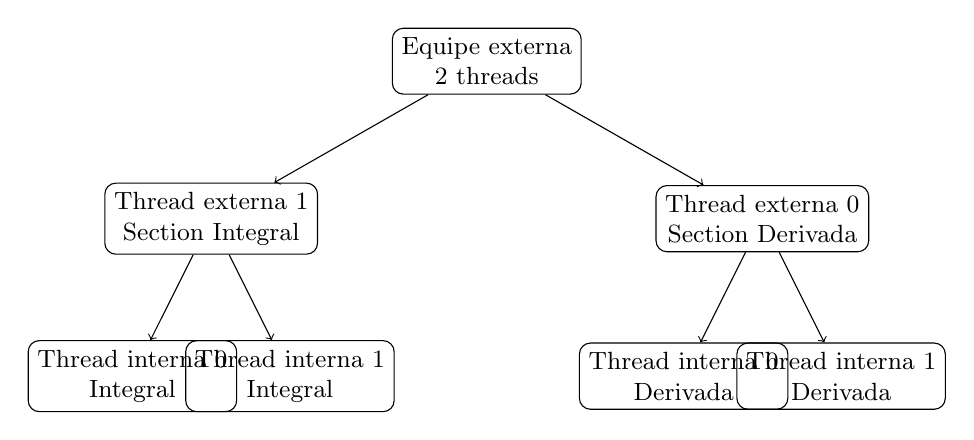
\begin{tikzpicture}[
        every node/.style={
            draw,
            rounded corners,
            align=center,
            minimum height=0.8cm,
            font=\small
        }
    ]

        \node (outer) at (0,0)
        {Equipe externa\\2 threads};

        \node (t1) at (-3.5,-2)
        {Thread externa 1\\Section Integral};

        \node (t0) at (3.5,-2)
        {Thread externa 0\\Section Derivada};

        \node (i0) at (-4.5,-4)
        {Thread interna 0\\Integral};

        \node (i1) at (-2.5,-4)
        {Thread interna 1\\Integral};

        \node (d0) at (2.5,-4)
        {Thread interna 0\\Derivada};

        \node (d1) at (4.5,-4)
        {Thread interna 1\\Derivada};

        \draw[->] (outer) -- (t1);
        \draw[->] (outer) -- (t0);

        \draw[->] (t1) -- (i0);
        \draw[->] (t1) -- (i1);

        \draw[->] (t0) -- (d0);
        \draw[->] (t0) -- (d1);

    \end{tikzpicture}

    \caption{Distribuição de threads observada na execução da Atividade 8.}
    \label{fig:atvd08-paralelismo-observado}
\end{figure}

É importante distinguir essa figura de uma regra fixa de escalonamento. Ela
documenta a execução observada; outra execução válida poderia inverter as
threads externas responsáveis pelas duas \texttt{sections}.


% ============================================================================
\section{Análise e discussão}
\label{sec:atvd08-discussao}
% ============================================================================

\subsection{Paralelismo de tarefas}

O paralelismo de tarefas foi explorado após a conclusão da inicialização.

Como integral e derivada utilizam o mesmo vetor de entrada, mas não dependem
dos resultados uma da outra, elas foram colocadas em duas diretivas
\texttt{section} distintas.

A execução observada demonstrou:

\begin{center}
\texttt{Integral} $\rightarrow$ thread externa 1
\end{center}

e

\begin{center}
\texttt{Derivada} $\rightarrow$ thread externa 0.
\end{center}

Esse resultado evidencia que a atribuição é responsabilidade do runtime e não
foi codificada manualmente.


\subsection{Paralelismo de dados}

O segundo nível de paralelismo aparece dentro das tarefas.

Na integral, as iterações responsáveis pelo somatório intermediário são
distribuídas entre as duas threads da equipe interna.

Na derivada, diferentes índices do vetor são distribuídos entre as threads.
Como cada iteração escreve em uma posição distinta de \texttt{dy}, não existe
conflito de escrita entre elas.

A inicialização do vetor também utiliza paralelismo de dados, pois cada
posição de \texttt{y} pode ser calculada independentemente.


\subsection{Paralelismo aninhado}

A execução confirmou que as duas regiões internas utilizaram equipes com duas
threads.

Isso é importante porque uma região paralela interna poderia ser serializada
caso o paralelismo aninhado não estivesse habilitado ou caso o runtime não
permitisse a criação de equipes adicionais.

O output:

\begin{center}
\texttt{Equipe interna : 2 threads}
\end{center}

para as duas tarefas fornece evidência direta de que as regiões internas
foram efetivamente ativadas no ambiente testado.


\subsection{Redução e ausência de condição de corrida}

O somatório da integral representa o principal ponto em que múltiplas threads
contribuem para uma mesma grandeza.

Uma implementação do tipo

\begin{center}
\texttt{sum += y[i]}
\end{center}

sobre uma única variável compartilhada, sem proteção, estaria sujeita a
condição de corrida.

A cláusula \texttt{reduction} evita esse problema criando estados parciais
privados e combinando-os posteriormente.

Essa estratégia também é mais apropriada do que proteger cada atualização
com uma seção crítica, pois uma região \texttt{critical} em cada iteração
serializaria a etapa de acumulação.


\subsection{Sincronização}

A solução utiliza predominantemente sincronização implícita.

O fim da região paralela da inicialização funciona como um ponto de junção:
somente depois dele o vetor pode ser consumido pelas tarefas.

As regiões paralelas internas também possuem um ponto de junção em seu
término.

A construção \texttt{sections}, utilizada sem \texttt{nowait}, possui
barreira implícita ao final. Esse comportamento é desejado porque o bloco
\texttt{single} que apresenta os resultados só deve executar depois que
integral e derivada estejam completas.

Assim, não foi necessário adicionar uma diretiva \texttt{barrier} manual.


\subsection{Impressão por uma única thread}

A impressão final ocorre no interior de uma construção \texttt{single}.

Dessa maneira, apesar de duas threads participarem da região externa, apenas
uma executa o bloco de saída.

A escolha também evita que integral e derivada realizem impressão concorrente
diretamente de suas respectivas \texttt{sections}, o que poderia tornar a
ordem visual do terminal não determinística e dificultar a leitura.


\subsection{Comportamento numérico da integral}

O erro absoluto observado foi da ordem de

\[
10^{-8}.
\]

Esse resultado é coerente com a discretização adotada e com o erro esperado
para o método dos trapézios aplicado à função quadrática.

A aproximação foi ligeiramente superior ao valor exato, comportamento
consistente com a convexidade de $x^2$.


\subsection{Comportamento numérico da derivada}

Nos pontos internos, a aproximação coincide com $2x$ na precisão exibida.

Isso não deve ser interpretado como uma propriedade universal do método de
diferenças finitas. Nesse caso específico, a diferença central aplicada a uma
função quadrática cancela exatamente os termos de erro de ordem superior
relevantes para o cálculo.

Já nas extremidades, as diferenças progressiva e regressiva são de primeira
ordem, razão pela qual foram observados:

\[
0{,}000100
\]

em $x=0$, em vez de zero, e

\[
19{,}999900
\]

em $x=10$, em vez de $20$.

Esses valores são consistentes com o espaçamento empregado.


\subsection{Relação entre correção e desempenho}

Apesar de utilizar paralelismo, a atividade não fornece evidência experimental
de que a versão paralela seja mais rápida do que uma versão sequencial.

O objetivo foi demonstrar corretamente a decomposição e a sincronização.

Qualquer afirmação sobre ganho de desempenho exigiria uma metodologia
adicional, incluindo versão sequencial de referência, variação do número de
threads, repetição das medições e análise estatística dos tempos.


% ============================================================================
\section{Limitações}
\label{sec:atvd08-limitacoes}
% ============================================================================

A primeira limitação é a ausência deliberada de temporização. A atividade
valida a estrutura paralela e a correção numérica, mas não permite avaliar
speedup, eficiência ou escalabilidade.

A segunda limitação é o uso de uma única função, um único intervalo e um único
tamanho de vetor. A escolha de $f(x)=x^2$ é apropriada para fins didáticos,
mas não representa toda a variedade de comportamentos possíveis em problemas
numéricos.

A terceira limitação decorre da própria construção \texttt{sections}. O
número de tarefas disponíveis é definido estaticamente no código, de modo que
esse mecanismo não é destinado a problemas com grande quantidade dinâmica de
tarefas.

A associação entre threads externas e \texttt{sections} também não é
determinística. A execução registrada atribuiu integral à thread 1 e derivada
à thread 0, mas essa associação não deve ser considerada requisito de
correção.

Os identificadores 0 e 1 das equipes internas são locais às respectivas
equipes OpenMP. Portanto, uma ``thread interna 0'' de uma tarefa não deve ser
interpretada simplesmente como a mesma entidade da ``thread interna 0'' de
outra equipe.

A soma em ponto flutuante realizada por redução também pode apresentar
pequenas diferenças nos últimos dígitos caso a ordem de combinação das
parcelas mude, pois a adição em ponto flutuante não é estritamente
associativa.

Outra limitação é o tratamento das extremidades da derivada com fórmulas
unilaterais de primeira ordem. Isso explica o erro maior nas extremidades em
comparação com os pontos internos.

A validação impressa da derivada utiliza somente cinco amostras
representativas. O vetor completo é calculado, mas não é integralmente
apresentado para evitar uma saída de $100000$ linhas.

Por fim, a versão exata do compilador GCC não foi registrada juntamente com o
output. A reprodutibilidade funcional é sustentada pelo comando de compilação
e pelo ambiente UCRT64 utilizado, mas uma reprodução estrita deveria também
registrar a versão do compilador e do runtime OpenMP.


% ============================================================================
\section{Conclusões da atividade}
\label{sec:atvd08-conclusao}
% ============================================================================

A Atividade 8 permitiu integrar, em uma única aplicação, três conceitos
centrais de programação paralela com OpenMP: paralelismo de tarefas,
paralelismo de dados e paralelismo aninhado.

A dependência entre as fases foi modelada explicitamente. A inicialização
ocorre antes das operações numéricas, enquanto integral e derivada são
executadas como tarefas independentes por meio de \texttt{sections}.

Cada tarefa cria sua própria região paralela com duas threads, atendendo ao
requisito de explorar paralelismo de dados dentro do paralelismo de tarefas.

A integral utiliza \texttt{reduction} para combinar as contribuições das
threads sem condição de corrida. A derivada distribui índices independentes
entre as threads sem necessidade de exclusão mútua.

A sincronização necessária é obtida predominantemente pelas barreiras
implícitas das construções OpenMP empregadas, e a apresentação final é
executada por apenas uma thread utilizando \texttt{single}.

A execução confirmou o funcionamento do paralelismo aninhado, com duas
threads internas tanto para a integral quanto para a derivada.

Numericamente, a integral apresentou erro absoluto de

\[
1{,}666609250606\times10^{-8},
\]

compatível com a discretização utilizada. Nos pontos internos da derivada, os
resultados coincidiram com $f'(x)=2x$ na precisão apresentada, enquanto os
pequenos desvios das extremidades foram consistentes com as diferenças
unilaterais adotadas.

Dessa forma, a implementação atende ao objetivo didático da atividade sem
introduzir mecanismos paralelos desnecessários ou conclusões de desempenho
não sustentadas experimentalmente.


% ============================================================================
\section{Síntese}
\label{sec:atvd08-defesa}
% ============================================================================

Para uma defesa oral da atividade, os pontos centrais podem ser sintetizados
da seguinte forma:

\begin{enumerate}

    \item A função escolhida foi $f(x)=x^2$, no intervalo $[0,10]$, com
    $100000$ pontos e valores do tipo \texttt{double}.

    \item A inicialização precisa terminar antes dos demais cálculos, pois
    integral e derivada dependem do vetor da função.

    \item Depois da inicialização, integral e derivada são independentes e,
    portanto, foram colocadas em duas \texttt{sections}.

    \item Esse nível externo representa paralelismo de tarefas.

    \item Uma \texttt{section} sozinha é executada por uma thread. Como o
    enunciado exige pelo menos duas threads por tarefa, cada \texttt{section}
    cria uma região paralela interna com duas threads.

    \item As regiões internas representam paralelismo de dados e caracterizam
    o paralelismo aninhado.

    \item Na integral, as threads dividem os termos do somatório. Como todas
    contribuem para uma única soma, foi usada
    \texttt{reduction(+:sum)} para evitar condição de corrida.

    \item Na derivada, cada thread escreve em índices diferentes do vetor de
    saída, portanto não é necessário \texttt{critical} ou \texttt{atomic}.

    \item A diferença central foi usada no interior do domínio; diferenças
    progressiva e regressiva foram usadas nas extremidades.

    \item O paralelismo aninhado foi habilitado explicitamente com
    \texttt{omp\_set\_nested(1)} e a alteração dinâmica do número de threads
    foi desabilitada com \texttt{omp\_set\_dynamic(0)}.

    \item Não foi necessário escrever uma \texttt{barrier} explícita. Foram
    utilizadas as sincronizações implícitas das regiões paralelas e de
    \texttt{sections}.

    \item A impressão final é protegida por \texttt{single}, garantindo que
    apenas uma thread apresente os resultados.

    \item Na execução observada, a integral foi atribuída à thread externa 1
    e a derivada à thread externa 0. Essa associação pode mudar em outra
    execução e não foi fixada no programa.

    \item As duas tarefas criaram equipes internas com as threads 0 e 1,
    confirmando que o paralelismo aninhado estava efetivamente ativo.

    \item A integral numérica obtida foi
    $333{,}333333349999$, contra
    $333{,}333333333333$ analítico, com erro absoluto de
    $1{,}666609250606\times10^{-8}$.

    \item Nos pontos internos, a derivada numérica coincidiu com $2x$ na
    precisão impressa. O pequeno erro nas extremidades decorre das diferenças
    unilaterais.

    \item Não foi realizado benchmark. Portanto, a atividade demonstra
    correção e organização do paralelismo, mas não permite afirmar ganho de
    desempenho.

\end{enumerate}
